\documentclass[11pt,compress,t,notes=noshow, xcolor=table]{beamer}
\usepackage[]{graphicx}\usepackage[]{color}
% maxwidth is the original width if it is less than linewidth
% otherwise use linewidth (to make sure the graphics do not exceed the margin)
\makeatletter
\def\maxwidth{ %
  \ifdim\Gin@nat@width>\linewidth
    \linewidth
  \else
    \Gin@nat@width
  \fi
}
\makeatother

\newcommand{\citebutton}[2]{%
\beamergotobutton{\href{#2}{#1}}%
}

\newcommand{\blu}[1]{\textcolor{blue}{#1}}
\newcommand{\org}[1]{\textcolor{orange}{#1}}
\newcommand{\ques}{\textbf{\textcolor{red}{Question:  }}}
\newcommand{\questionssofar}{\begin{frame}\frametitle{Any questions?}\end{frame}}

\newcommand\warning{%
 \makebox[1.4em][c]{%
 \makebox[0pt][c]{\raisebox{.1em}{\scriptsize!}}%
 \makebox[0pt][c]{\color{red}\normalsize$\bigtriangleup$}}}%

\definecolor{fgcolor}{rgb}{0.345, 0.345, 0.345}
\newcommand{\hlnum}[1]{\textcolor[rgb]{0.686,0.059,0.569}{#1}}%
\newcommand{\hlstr}[1]{\textcolor[rgb]{0.192,0.494,0.8}{#1}}%
\newcommand{\hlcom}[1]{\textcolor[rgb]{0.678,0.584,0.686}{\textit{#1}}}%
\newcommand{\hlopt}[1]{\textcolor[rgb]{0,0,0}{#1}}%
\newcommand{\hlstd}[1]{\textcolor[rgb]{0.345,0.345,0.345}{#1}}%
\newcommand{\hlkwa}[1]{\textcolor[rgb]{0.161,0.373,0.58}{\textbf{#1}}}%
\newcommand{\hlkwb}[1]{\textcolor[rgb]{0.69,0.353,0.396}{#1}}%
\newcommand{\hlkwc}[1]{\textcolor[rgb]{0.333,0.667,0.333}{#1}}%
\newcommand{\hlkwd}[1]{\textcolor[rgb]{0.737,0.353,0.396}{\textbf{#1}}}%
\let\hlipl\hlkwb

\usepackage{framed}
\makeatletter
\newenvironment{kframe}{%
 \def\at@end@of@kframe{}%
 \ifinner\ifhmode%
  \def\at@end@of@kframe{\end{minipage}}%
  \begin{minipage}{\columnwidth}%
 \fi\fi%
 \def\FrameCommand##1{\hskip\@totalleftmargin \hskip-\fboxsep
 \colorbox{shadecolor}{##1}\hskip-\fboxsep
     % There is no \\@totalrightmargin, so:
     \hskip-\linewidth \hskip-\@totalleftmargin \hskip\columnwidth}%
 \MakeFramed {\advance\hsize-\width
   \@totalleftmargin\z@ \linewidth\hsize
   \@setminipage}}%
 {\par\unskip\endMakeFramed%
 \at@end@of@kframe}
\makeatother

\definecolor{shadecolor}{rgb}{.97, .97, .97}
\definecolor{messagecolor}{rgb}{0, 0, 0}
\definecolor{warningcolor}{rgb}{1, 0, 1}
\definecolor{errorcolor}{rgb}{1, 0, 0}
\newenvironment{knitrout}{}{} % an empty environment to be redefined in TeX

\usepackage{alltt}
\newcommand{\SweaveOpts}[1]{}  % do not interfere with LaTeX
\newcommand{\SweaveInput}[1]{} % because they are not real TeX commands
\newcommand{\Sexpr}[1]{}       % will only be parsed by R
\newcommand{\xmark}{\ding{55}}%


\usepackage[english]{babel}
\usepackage[utf8]{inputenc}

\usepackage{dsfont}
\usepackage{verbatim}
\usepackage{amsmath}
\usepackage{amsfonts}
\usepackage{amssymb}
\usepackage{bm}
\usepackage{csquotes}
\usepackage{multirow}
\usepackage{longtable}
\usepackage{booktabs}
\usepackage{enumerate}
\usepackage[absolute,overlay]{textpos}
\usepackage{psfrag}
\usepackage{algorithm}
\usepackage{algpseudocode}
\usepackage{eqnarray}
\usepackage{arydshln}
\usepackage{tabularx}
\usepackage{placeins}
\usepackage{tikz}
\usepackage{setspace}
\usepackage{colortbl}
\usepackage{mathtools}
\usepackage{wrapfig}
\usepackage{bm}
\usepackage{amsmath}
\usepackage{pifont}

\usetikzlibrary{shapes.multipart,shapes,arrows,automata,positioning,calc,chains,trees, shadows}
\tikzset{
  %Define standard arrow tip
  >=stealth',
  %Define style for boxes
  punkt/.style={
    rectangle,
    rounded corners,
    draw=black, very thick,
    text width=6.5em,
    minimum height=2em,
    text centered},
  % Define arrow style
  pil/.style={
    ->,
    thick,
    shorten <=2pt,
    shorten >=2pt,}
}

\tikzstyle{vec}=[draw, rectangle, fill = white, minimum width=5mm, minimum height=1cm, inner sep = 2pt]

\usepackage{subfig}

% Defines macros and environments
\usepackage{../../style/lmu-lecture}


\let\code=\texttt
\let\proglang=\textsf

\setkeys{Gin}{width=0.9\textwidth}

\setbeamertemplate{frametitle}{\expandafter\uppercase\expandafter\insertframetitle}

\usepackage{bbm}
% basic latex stuff
\newcommand{\pkg}[1]{{\fontseries{b}\selectfont #1}} %fontstyle for R packages
\newcommand{\lz}{\vspace{0.5cm}} %vertical space
\newcommand{\dlz}{\vspace{1cm}} %double vertical space
\newcommand{\oneliner}[1] % Oneliner for important statements
{\begin{block}{}\begin{center}\begin{Large}#1\end{Large}\end{center}\end{block}}


%new environments
\newenvironment{vbframe}  %frame with breaks and verbatim
{
 \begin{frame}[containsverbatim,allowframebreaks]
}
{
\end{frame}
}

\newenvironment{vframe}  %frame with verbatim without breaks (to avoid numbering one slided frames)
{
 \begin{frame}[containsverbatim]
}
{
\end{frame}
}

\newenvironment{blocki}[1]   % itemize block
{
 \begin{block}{#1}\begin{itemize}
}
{
\end{itemize}\end{block}
}

\newenvironment{fragileframe}[2]{  %fragile frame with framebreaks
\begin{frame}[allowframebreaks, fragile, environment = fragileframe]
\frametitle{#1}
#2}
{\end{frame}}


\newcommand{\myframe}[2]{  %short for frame with framebreaks
\begin{frame}[allowframebreaks]
\frametitle{#1}
#2
\end{frame}}

\newcommand{\remark}[1]{
  \textbf{Remark:} #1
}


\newenvironment{deleteframe}
{
\begingroup
\usebackgroundtemplate{
\includegraphics[width=\paperwidth,height=\paperheight]{../style/color/red.png}}
 \begin{frame}
}
{
\end{frame}
\endgroup
}
\newenvironment{simplifyframe}
{
\begingroup
\usebackgroundtemplate{
\includegraphics[width=\paperwidth,height=\paperheight]{../style/color/yellow.png}}
 \begin{frame}
}
{
\end{frame}
\endgroup
}\newenvironment{draftframe}
{
\begingroup
\usebackgroundtemplate{
\includegraphics[width=\paperwidth,height=\paperheight]{../style/color/green.jpg}}
 \begin{frame}
}
{
\end{frame}
\endgroup
}
% https://tex.stackexchange.com/a/261480: textcolor that works in mathmode
\makeatletter
\renewcommand*{\@textcolor}[3]{%
  \protect\leavevmode
  \begingroup
    \color#1{#2}#3%
  \endgroup
}
\makeatother





\input{../../latex-math/basic-math.tex}
\input{../../latex-math/basic-ml.tex}

\tikzstyle{squ}=[draw, rectangle, minimum size = 5mm]
\tikzstyle{del}=[squ, fill = white]

\newcommand{\titlefigure}{figure/attn.png}
\newcommand{\learninggoals}{
\item Understand attention mechanism
\item Learn the different types of attention}

\title{Deep Learning Basics}
% \author{}
\institute{\href{https://slds-lmu.github.io/lecture_dl4nlp/}{slds-lmu.github.io/lecture\_dl4nlp}}
\date{}

\begin{document}
\lecturechapter{Attention}
\lecture{Deep Learning for NLP}

% ------------------------------------------------------------------------------

\begin{vbframe}{Encoder-Decoder with RNNs}

\vskip-3mm
\vfill

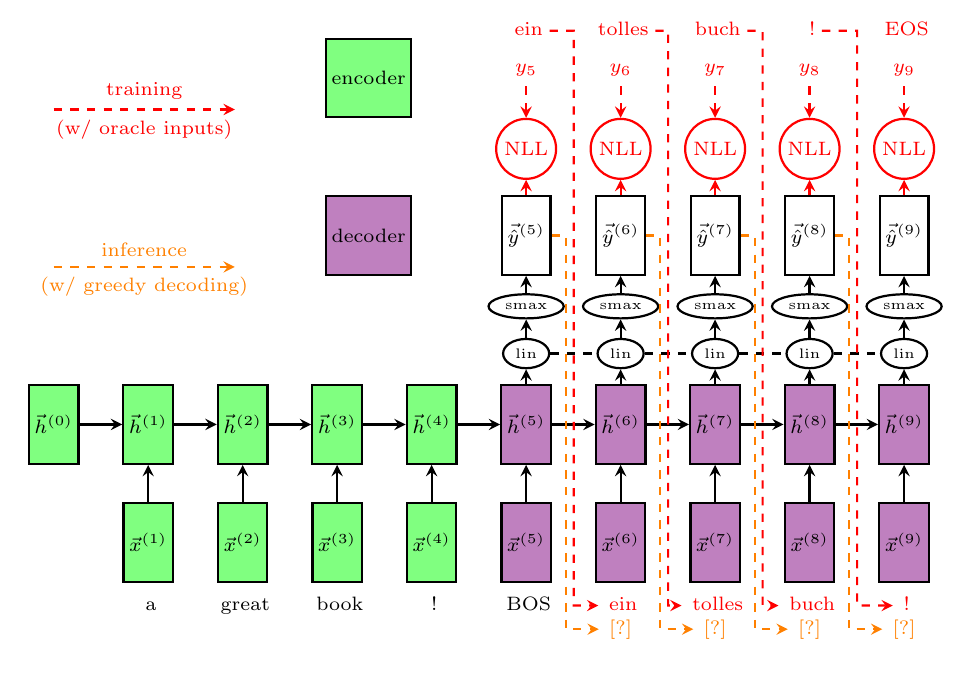
\begin{tikzpicture}[->, thick, >=stealth]
\node [vec, fill=green!50] (h0) at (0,2) {\scriptsize $\vec h^{(0)}$};
\foreach \i/\word/\coll in {1/a/green,2/great/green,3/book/green,4/!/green,5/BOS/violet,6/ein/violet,7/tolles/violet,8/buch/violet,9/!/violet}{
\node [vec, fill=\coll!50] (x\i) at (\i*1.2, .5) {\scriptsize $\vec x^{(\i)}$};
\node [vec, fill=\coll!50] (h\i) at (\i*1.2, 2) {\scriptsize $\vec h^{(\i)}$};
\draw (x\i) -- (h\i);
\pgfmathparse{\i-1};
\draw (h\pgfmathresult) -- (h\i);
}
\foreach \i/\word/\coll in {1/a/green,2/great/green,3/book/green,4/!/green,5/BOS}{
\node (in\i) [text=black, inner sep=-2pt, outer sep=0pt] at (\i*1.2,-.3) {\scriptsize \phantom{A}\word\phantom{g}};
}

\foreach \i/\word/\coll in {6/ein/violet,7/tolles/violet,8/buch/violet,9/!/violet}{
\node (in\i) [text=red, inner sep=-2pt, outer sep=0pt] at (\i*1.2,-.3) {\scriptsize \phantom{A}\word\phantom{g}};
}

\foreach \i/\word in {5/ein,6/tolles,7/buch,8/!,9/EOS}{
\node (smax\i) [draw, ellipse, inner sep=2pt] at (\i*1.2, 3.5) {\tiny smax};
\node (ffn\i) [draw, ellipse, inner sep=2pt] at (\i*1.2, 2.9) {\tiny lin};
\node (pred\i) [vec] at (\i*1.2, 4.4) {\scriptsize $\vec {\hat{y}}^{(\i)}$};
\node (lab\i) [red] at (\i*1.2, 6.5) {\scriptsize ${y}_\i$};
\node (loss\i) [draw, circle, inner sep=2pt, red] at (\i*1.2, 5.5) {\scriptsize NLL};
\node (out\i) [text=red, inner sep=-2pt] at (\i*1.2,7) {\scriptsize \phantom{A}\word\phantom{g}};
\draw  (h\i) -- (ffn\i);
\draw (ffn\i) -- (smax\i);
\draw  (smax\i) -- (pred\i);
\draw (pred\i) [dashed, red] -- (loss\i);
\draw  (lab\i) [dashed, red] -- (loss\i);
}
\draw [dashed, -] (ffn5)--(ffn6)--(ffn7)--(ffn8)--(ffn9);

\draw [dashed, orange] (0, 4) -- node[midway, above, font=\scriptsize] {inference} (2.3,4);
\draw [orange, draw=none] (0, 4) -- node[midway, below, font=\scriptsize] {(w/ greedy decoding)} (2.3,4);
\draw [dashed, red] (0, 6) -- node[midway, above, font=\scriptsize] {training} (2.3,6);
\draw [red, draw=none] (0, 6) -- node[midway, below, font=\scriptsize] {(w/ oracle inputs)} (2.3,6);

\node [vec, fill=green!50] at (4, 6.4) {\scriptsize encoder};
\node [vec, fill=violet!50] at (4, 4.4) {\scriptsize decoder};

\foreach \j/\t in {6/5,7/6,8/7,9/8}{
\pgfmathparse{\j-1};
\node (argmax\j) [text=orange] at (\j*1.2,-.6) {\scriptsize [?]};
\node [xshift=-1.5mm] (pt\j) at ($(ffn\pgfmathresult)!0.5!(ffn\j)$) {};
\node [xshift=-2.5mm] (px\j) at ($(ffn\pgfmathresult)!0.5!(ffn\j)$) {};
\draw [dashed, red] (out\pgfmathresult) -- (pt\j |- out\pgfmathresult) -- (pt\j |- in\j) -- (in\j);
\draw [dashed, orange] (pred\pgfmathresult) -- (px\j |- pred\pgfmathresult) -- (px\j |- argmax\j) -- (argmax\j);
}
\end{tikzpicture}

\vfill

\end{vbframe}

% ------------------------------------------------------------------------------

\begin{vbframe}{Other Encoder-Decoder Applications}

\vfill

\begin{itemize}
	\item Text summarization
	\item Text generation
	\item Keyword generation
	\item Automatic speech recognition
	\item Subtitle generation
	\item Question answering
	\item Named entity recognition
	\item Video or image captioning
	\item Part-of-speech tagging
	\item ...more
\end{itemize}

\vfill

\end{vbframe}

% ------------------------------------------------------------------------------

\begin{vbframe}{Limitations of RNNs}

\vfill

\begin{itemize}
	\item In an RNN, at a given point in time $j$, the information about all past inputs $x^{(1)} \ldots x^{(j)}$ is ``crammed'' into the state vector $\vec h^{(j)}$ (and $\vec c^{(j)}$ for an LSTM)
	\item So for long sequences, the state becomes a \textbf{bottleneck}
	\item Especially problematic in encoder-decoder models (e.g., for Machine Translation)
	\item Solution: Attention \beamergotobutton{\href{https://arxiv.org/abs/1409.0473}{Bahdanau et al., 2015}} -- an architectural modification of the RNN encoder-decoder that allows the model to ``attend to'' past encoder states
\end{itemize}

\vfill

\end{vbframe}

% ------------------------------------------------------------------------------

\begin{frame}{bahdanau attention}
	
\vfill

\begin{figure}
	\centering
		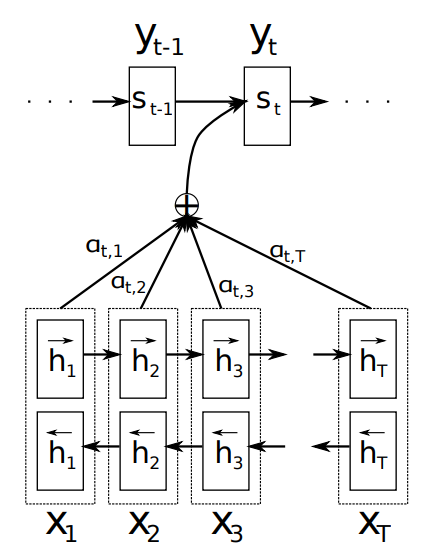
\includegraphics[width = 5.5cm]{figure/bahdanau-attention.png}\\ 
	\beamergotobutton{\href{https://arxiv.org/abs/1409.0473}{Source: Bahdanau et al., 2015}}
\end{figure}

\vfill
	
\end{frame}

% ------------------------------------------------------------------------------

\begin{vbframe}{Attention: The basic recipe (1)}

\vfill

\begin{itemize}
	\item \textbf{Ingredients:}
	\item[]
	\item One query vector: $\mathbf{q} \in \mathbb{R}^{d_q}$
	\item J key vectors: $\mathbf{K} \in \mathbb{R}^{J \times d_k}; (\vec k_1 \ldots \vec k_J)$
	\item J value vectors: $\mathbf{V} \in \mathbb{R}^{J \times d_v}; (\vec v_1 \ldots \vec v_J)$
	\item Scoring function $a : \mathbb{R}^{d_q} \times \mathbb{R}^{d_k} \rightarrow \mathbb{R}$
		\begin{itemize}
			\item Maps a query-key pair to a scalar (``score'')
			\item $a$ may be parametrized by parameters $\theta_a$
		\end{itemize}
\end{itemize}

\vfill

\end{vbframe}

% ------------------------------------------------------------------------------

\begin{vbframe}{Attention: The basic recipe (2)}

\vfill

\begin{itemize}
	\item \textbf{Step 1}: Apply $a$ to $\vec q$ and all keys $\vec k_j$ to get scores (one per key): 
	$$\vec e = \begin{bmatrix} e_1 \\ \vdots \\ e_J \end{bmatrix} =  \begin{bmatrix} a(\vec q, \vec k_1; \theta_a) \\ \vdots \\ a(\vec q, \vec k_J; \theta_a) \end{bmatrix}$$
	\item \textbf{Step 2}: Turn $\mathbf{e}$ into a probability distribution with the softmax function
	$$\alpha_j = \frac{\mathrm{exp}(e_j)}{\sum_{j'=1}^J \mathrm{exp}(e_{j'})}$$
		\begin{itemize}
			\item Note that $\sum_j \alpha_j = 1$
		\end{itemize}
\end{itemize}

\vfill

\end{vbframe}

% ------------------------------------------------------------------------------

\begin{vbframe}{Attention: The basic recipe (3)}

\vfill

\begin{itemize}
	\item \textbf{Step 3}: $\alpha$-weighted sum over $\vec {V}$ yields one $d_v$-dimensional output vector:
	$$\vec {o} = \sum_{j=1}^J \alpha_j \vec {v}_j$$
		\begin{itemize}
			\item Intuition: $\alpha_j$ is how much ``attention'' the model pays to $\vec v_j$ when computing $\vec o$.
		\end{itemize}
\end{itemize}

\vfill

\end{vbframe}

% ------------------------------------------------------------------------------

\begin{vbframe}{Attention: An analogy (1)}

\vfill

\begin{itemize}
\item We have $J$ weather stations on a map
\item $\vec K \in \mathbb{R}^{J\times 2}$ are their geolocations (x,y coordinates)
\item $\vec V \in \mathbb{R}^{J \times d_v}$ are their current weather conditions (temperature, humidity, etc.)
\item $\vec q \in \mathbb{R}^2$ is a new geolocation for which we want to estimate weather conditions
\item $e_j$ is the relevance of the $j$'th station (e.g., $e_j = a(\vec q, \vec k_j) = \frac{1}{||\vec q - \vec k_j||_2}$), and $\alpha_j$ is $e_j$ as a probability
\end{itemize}

\vfill

\end{vbframe}

% ------------------------------------------------------------------------------

\begin{vbframe}{Attention: An analogy (2)}

\vfill

\begin{itemize}
\item $\vec o$: a weighted sum of all known weather conditions, where stations that have a small distance (high $\alpha$) have a higher weight
\begin{center}
\begin{tikzpicture}
\node (map) at (0,0){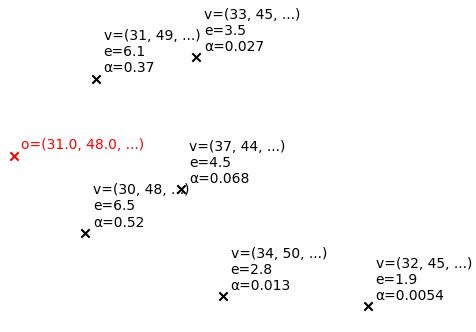
\includegraphics[width=.7\textwidth]{figure/map}};
\node (q) [left=1cm of map, red] {x: $\vec q$};
\node [below=2mm of q, black] {x: $\vec k_j$};
\end{tikzpicture}
\end{center}
\end{itemize}

\vfill

\end{vbframe}

% ------------------------------------------------------------------------------

\begin{vbframe}{Attention in neural networks}

\vskip-2mm
\vfill

\begin{itemize}
\item Contrary to our geolocation example, the $\vec q$, $\vec k_j$ and $\vec v_j$ vectors of a neural network are a function of the input and trainable parameters
\item So the \textit{model} learns which keys are relevant for which queries, based on the training data and loss function
\end{itemize}

\begin{figure}
	\centering
		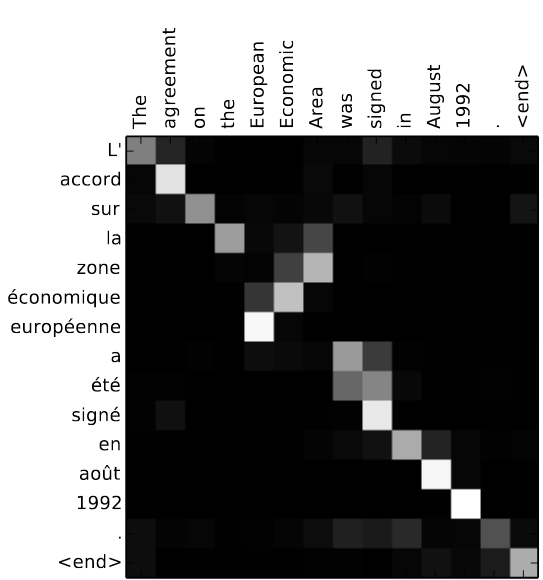
\includegraphics[width = 4.5cm]{figure/bahdanau4.png}\\ 
	\beamergotobutton{\href{https://arxiv.org/abs/1409.0473}{Source: Bahdanau et al., 2015}}
\end{figure}

\vfill

\end{vbframe}

% ------------------------------------------------------------------------------

\begin{vbframe}{A Primer on the Transformer (1)}

\vfill

\begin{itemize}
	\item The Bahdanau model is still an RNN, just with attention on top.
	\item Another architecture that consists of attention only: 
		\begin{itemize}
			\item Transformer: ``Attention is all you need'' \beamergotobutton{\href{https://arxiv.org/abs/1706.03762}{Vaswani et al., 2017}}
			\item No recurrence, \textit{just} Attention (as the name suggests)
			\item Better parallelizable (as opposed to RNNs)
			\item Will be introduced in chapter 3
		\end{itemize}
\end{itemize}

\vfill

\end{vbframe}

% ------------------------------------------------------------------------------

\begin{vbframe}{A Primer on the Transformer (2)}

\vfill

\begin{itemize}
	\item No (or few) assumptions are baked into the architecture (no notion of which words are neighbors in the sentence, sequentiality, etc.)
	\item The lack of prior knowledge often means that the Transformer requires more training data than an RNN to achieve a certain performance
	\item But when presented with sufficient data, it usually outperforms them
\end{itemize}

\vfill

\end{vbframe}

% ------------------------------------------------------------------------------

\endlecture
\end{document}

% ------------------------------------------------------------------------------

\begin{vbframe}{The Transformer architecture (2)}

\vskip-3mm
\vfill

\begin{center}
\begin{tikzpicture}[->, >=stealth, thick, font=\scriptsize]
\node (transformer) at (0,0) {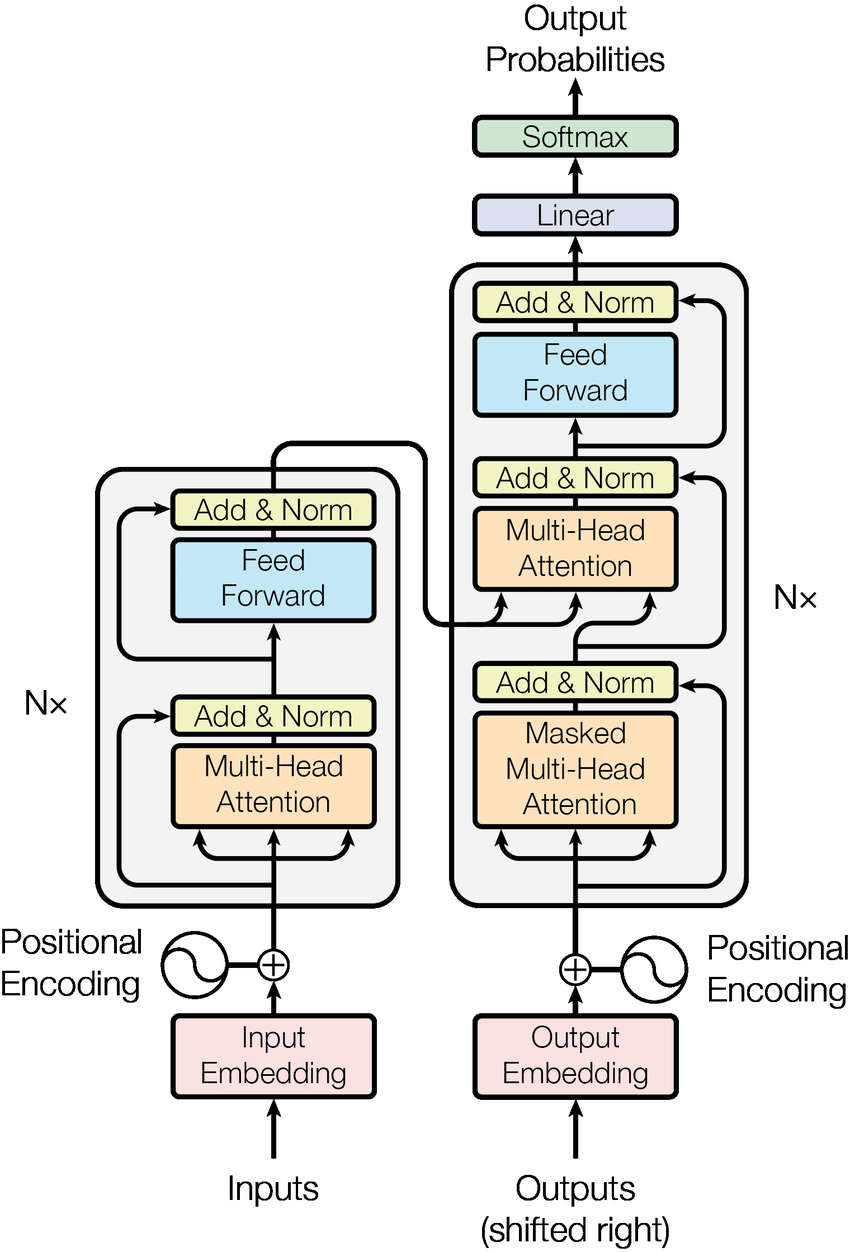
\includegraphics[width=.4\textwidth]{figure/transformer}};
\node (enc) [left=2mm of transformer, rotate=90] {encoder};
\node (dec) [right=2mm of transformer, rotate=270] {decoder};
\node (x) [above left=1cm of transformer.south west] {$X$ (source)};
\node (y) [above right=1cm of transformer.south east] {$Y$ (target)};
\draw (x) -- ([yshift=5mm, xshift=1cm] transformer.south west);
\draw (y) -- ([yshift=5mm, xshift=-1cm] transformer.south east);
\node (nll) [draw, circle] at ([yshift=-5mm] transformer.north east) {NLL};
\draw [bend right=55] (y.north east) to (nll);
\draw ([xshift=-1cm, yshift=-5mm] transformer.north east) to (nll);
\node at (-3, 2) [align=left] {(For simpler problems (e.g., \\ classification, tagging), \\ you would simply use \\ the encoder.)};
\end{tikzpicture}
\end{center}
{\scriptsize Figure from Vaswani et al. 2017: Attention is all you need}

\vfill

\end{vbframe}

% ------------------------------------------------------------------------------

\begin{vbframe}{Cross-attention and self-attention}

\vskip-3mm
\vfill

\begin{itemize}
	\item We can use attention on many different ``things'', including: 
		\begin{itemize}
			\item The pixels of images
			\item The nodes of knowledge graphs
			\item The words of a vocabulary
		\end{itemize}
	\item Here, we focus on scenarios where the query, key and value vectors represent tokens (e.g., words, characters, etc.) in sequences (e.g., sentences, paragraphs, etc.).
	\item Cross-attention:
		\begin{itemize}
			\item Let $X = (x_1 \ldots x_{J_x}), Y = (y_1 \ldots y_{J_y})$ be two sequences (e.g., source and target in a sequence-to-sequence problem)
			\item The query vectors represent tokens in $Y$ and the key/value vectors represent tokens in $X$ (``$Y$ attends to $X$'')
		\end{itemize}
	\item Self-attention:
		\begin{itemize}
			\item There is only one sequence $X = (x_1 \ldots x_J)$
			\item The query, key and value vectors represent tokens in $X$ (``$X$ attends to itself'')
		\end{itemize}
\end{itemize}

\vfill

\end{vbframe}

% ------------------------------------------------------------------------------

\begin{vbframe}{Cross-attention (1)}

\vfill

\begin{itemize}
	\item Here, we describe cross-attention. Self-attention can easily be derived by assuming $\vec X = \vec Y$. 
	\item Let $\vec X \in \mathbb{R}^{J_x \times d_x}, \vec Y \in \mathbb{R}^{J_y \times d_y}$ be representations of $X, Y$ (e.g., stacked word embeddings, or the outputs of a previous layer)
	\item Let $\theta = \{\vec W^{(q)} \in \mathbb{R}^{d_y \times d_q}, \vec W^{(k)} \in \mathbb{R}^{d_x \times d_k}, \vec W^{(v)} \in \mathbb{R}^{d_x \times d_v}\}$ be trainable weight matrices
	\item We transform $\vec Y$ into a matrix of query vectors:
	$$ \vec Q = \vec Y \vec W^{(q)} $$
	\item We transform $\vec X$ into matrices of key and value vectors:
	$$ \vec K = \vec X \vec W^{(k)} ; \qquad \vec V =  \vec X \vec W^{(v)}$$
\end{itemize}

\vfill

\end{vbframe}

% ------------------------------------------------------------------------------

\begin{vbframe}{Cross-attention (2)}

\vfill

\begin{itemize}
	\item To calculate the $e$ scores (step 1 of the basic recipe), Vaswani et al. use a parameter-less scaled dot product instead of Bahdanau's complicated FFN:
	$$ e_{j,j'} = a(\vec q_j, \vec k_{j'}) = \frac{\vec q_j^T \vec k_{j'}}{\sqrt{d_k}} $$
	\item Note: This requires that $d_q = d_k$
	\item Attention weights and outputs are defined like before (steps 2 and 3 of the basic recipe):
	$$ \alpha_{j,j'} = \frac{\mathrm{exp}(e_{j,j'})}{\sum_{j'' = 1}^{J_x} \mathrm{exp}(e_{j,j''})}$$
	$$ \vec o_j = \sum_{j'=1}^{J_x} \alpha_{j,j'} \vec v_{j'}$$
\end{itemize}

\vfill

\end{vbframe}

% ------------------------------------------------------------------------------

\begin{vbframe}{Cross-attention (3)}

\vskip-2mm
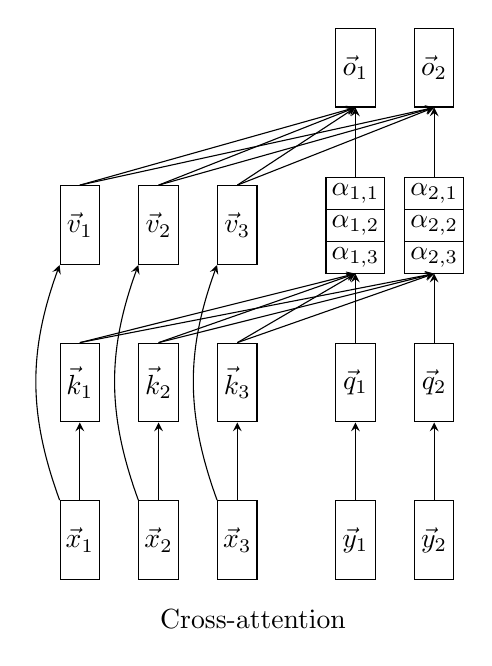
\begin{tikzpicture}[->, >=stealth]
\foreach \x in {1,2,3}{
\node (x\x) [vec] at (\x, -.5) {$\vec x_\x$};
\node (k\x) [vec] at (\x, 1.5) {$\vec k_\x$};
\node (v\x) [vec] at (\x, 3.5) {$\vec v_\x$};
}
\foreach \y in {1,2}{
\node (y\y) [vec] at (\y+3.5, -.5) {$\vec y_\y$};
\node (q\y) [vec] at (\y+3.5,1.5) {$\vec q_\y$};
\node (o\y) [vec] at (\y+3.5,5.5) {$\vec o_\y$};
\node (alpha\y) [vec, rectangle split, rectangle split parts=3] at (\y+3.5,3.5) {\nodepart{one} $\alpha_{\y,1}$ \nodepart{two} $\alpha_{\y,2}$ \nodepart{three} $\alpha_{\y,3}$};
}

\foreach \y in {1,2}{
\draw (alpha\y.north) -- (o\y.south);
\draw (q\y.north) -- (alpha\y.south);
\draw (y\y.north) -- (q\y.south);
\foreach \x in {1,2,3}{
\draw (v\x.north) -- (o\y.south);
\draw (k\x.north) -- (alpha\y.south);
}}
\foreach \x in {1,2,3}{
\draw (x\x.north) -- (k\x.south);
\draw [bend left=20] (x\x.north west) to (v\x.south west);
}
\node at (3.2, -1.5) {Cross-attention};
\end{tikzpicture}

\end{vbframe}

% ------------------------------------------------------------------------------

\begin{vbframe}{Cross-attention (4)}

\vskip-2mm
\hfill
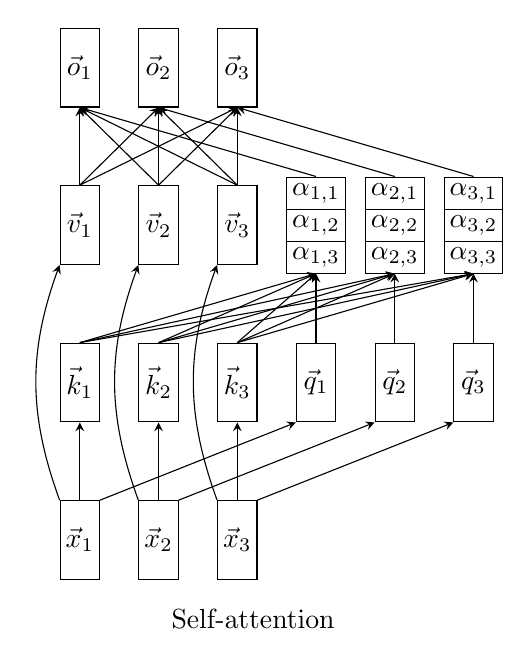
\begin{tikzpicture}[->, >=stealth]
\foreach \x in {1,2,3}{
\node (x\x) [vec] at (\x, -.5) {$\vec x_\x$};
\node (k\x) [vec] at (\x, 1.5) {$\vec k_\x$};
\node (v\x) [vec] at (\x, 3.5) {$\vec v_\x$};
}
\foreach \y in {1,2,3}{
\node (q\y) [vec] at (\y+3,1.5) {$\vec q_\y$};
\node (o\y) [vec] at (\y,5.5) {$\vec o_\y$};
\node (alpha\y) [vec, rectangle split, rectangle split parts=3] at (\y+3,3.5) {\nodepart{one} $\alpha_{\y,1}$ \nodepart{two} $\alpha_{\y,2}$ \nodepart{three} $\alpha_{\y,3}$};
}

\foreach \y in {1,2,3}{
\draw (alpha\y.north) -- (o\y.south);
\draw (q\y.north) -- (alpha\y.south);
\draw (x\y.north east) -- (q\y.south west);
\foreach \x in {1,2,3}{
\draw (v\x.north) -- (o\y.south);
\draw (k\x.north) -- (alpha\y.south);
}}
\foreach \x in {1,2,3}{
\draw (x\x.north) -- (k\x.south);
\draw [bend left=20] (x\x.north west) to (v\x.south west);
}
\node at (3.2, -1.5) {Self-attention};
\end{tikzpicture}

\end{vbframe}

% ------------------------------------------------------------------------------

\begin{vbframe}{Parallelized attention (1)}

\vfill

\begin{itemize}
	\item We want to apply our attention recipe to every query vector $\vec q_j$
	\item We could simply loop over all time steps $1 \leq j \leq J_y$ and calculate each $\vec o_j$ independently.
	\item Then stack all $\vec o_j$ into an output matrix $\vec O \in \mathbb{R}^{J_y \times d_v}$
	\item But a loop does not use the GPU's capacity for parallelization
	\item So it might be unnecessarily slow
\end{itemize}

\vfill

\end{vbframe}

% ------------------------------------------------------------------------------

\begin{vbframe}{Parallelized attention (2)}

\vfill

\begin{itemize}
\item Do some inputs (e.g., $\vec q_j$) depend on previous outputs (e.g., $\vec o_{j-1}$)? If not, we can parallelize the loop into a single function:
$$\vec O = \mathcal{F}^\mathrm{attn}(\vec X, \vec Y; \theta)$$
\item Attention in Transformers is usually parallelizable, unless we are doing autoregressive inference (more on that later).
\item By the way: The Bahdanau model is not parallelizable in this way, because $s_i$ (a.k.a. the query of the $i+1$'st step) depends on $c_i$ (a.k.a. the attention output of the $i$'th step), see last lecture:
\begin{center}
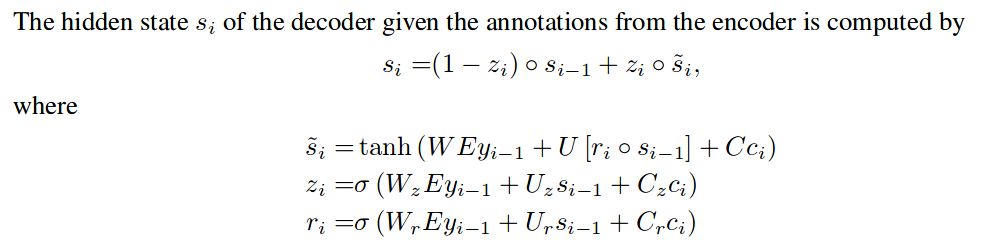
\includegraphics[width=.9\textwidth]{figure/bahdanau3}
\end{center}
\end{itemize}

\vfill

\end{vbframe}

% ------------------------------------------------------------------------------

\begin{vbframe}{Parallelized scaled dot product attention (1)}

\vfill 

\begin{itemize}
\item \textbf{Step 1}: The parallel application of the scaled dot product to all query-key pairs can be written as:
$$\vec {E} = \frac{ \vec {Q} \vec {K}^T}{\sqrt{d_k}}; \quad \vec E \in \mathbb{R}^{J_y \times J_x}$$
$$ \begin{matrix} \downarrow \\ queries \\ \downarrow \\ \end{matrix} \overset{\rightarrow keys \rightarrow}{
\begin{bmatrix}
e_{1,1} & \ldots & e_{1,J_x} \\
\vdots & \ddots & \vdots \\
e_{J_y,1} & \ldots & e_{J_y,J_x} \\
\end{bmatrix}} = \frac{1}{\sqrt{d_k}}
\begin{bmatrix} 
- & \vec q_1  & -  \\
& \vdots & \\
-  & \vec q_{J_y}  &  -  \\
\end{bmatrix}  
\begin{bmatrix} 
\lvert &  & \lvert  \\
\vec k_1 & \ldots & \vec k_{J_x} \\
\lvert &  & \lvert  \\
\end{bmatrix}$$
\end{itemize}

\vfill

\end{vbframe}

% ------------------------------------------------------------------------------

\begin{vbframe}{Parallelized scaled dot product attention (2)}

\vfill

\begin{itemize}
\item \textbf{Step 2}: Softmax with normalization over the second axis (key axis): 
$$\alpha_{j,j'} = \frac{\mathrm{exp}(e_{j,j'})}{\sum_{j''=1}^{J_x} \mathrm{exp}(e_{j,j''})}$$
\begin{verbatim}
>>> A = np.exp(E) / np.exp(E).sum(axis=-1, keepdims=True)
\end{verbatim}
\item Let's call this new normalized matrix $\vec A \in (0,1)^{J_y \times J_x}$
\item The rows of $\vec A$, denoted $\vec \alpha_j$, are probability distributions (one $\vec \alpha_j$ per $\vec q_j$)
\end{itemize}

\vfill

\end{vbframe}

% ------------------------------------------------------------------------------

\begin{vbframe}{Parallelized scaled dot product attention (3)}

\vfill

\begin{itemize}
\item \textbf{Step 3}: Weighted sum
$$\vec {O} = \vec {A} \vec {V}; \vec O \in \mathbb{R}^{J_y \times d_v}$$

$$
\begin{matrix} \downarrow \\ queries \\ \downarrow \end{matrix}
	\overset{\rightarrow d_v \text{(value dims)} \rightarrow}{
\begin{bmatrix}
o_{1,1} & \ldots & o_{1,d_v} \\
\vdots & \ddots & \vdots \\
o_{J_y,1} & \ldots & o_{J_y,d_v} \\
\end{bmatrix}} =
\begin{bmatrix} 
- & \boldsymbol \alpha_1  & -  \\
& \vdots & \\
-  & \boldsymbol \alpha_{J_y}  &  -  \\
\end{bmatrix}  
\begin{bmatrix} 
\lvert &  & \lvert  \\
\vec {v}_{:,1} & \ldots & \vec {v}_{:,d_v} \\
\lvert &  & \lvert  \\
\end{bmatrix}
$$
\end{itemize}

\vfill

\end{vbframe}

% ------------------------------------------------------------------------------

\begin{vbframe}{... as a one-liner}

\vfill

\large
$$ \vec O = \mathcal{F}^\mathrm{attn}(\vec X, \vec Y; \theta) = \mathrm{softmax}\Big(\frac{(\vec Y\vec W^{(q)} ) (\vec X\vec W^{(k)} )^T}{\sqrt{d_k}}\Big)(\vec X\vec W^{(v)} ) $$
\begin{itemize}
	\item GPUs like matrix multiplications $\rightarrow$ usually a lot faster than RNN!
	\item But: The memory requirements of $\vec E$ and $\vec A$ are $\mathcal{O}(J_y J_x)$
	\item A length up to about 500 is usually ok on a medium-sized GPU (and most sentences are shorter than that anyway).
	\item But when we consider inputs that span several sentences (e.g., paragraphs or whole documents), we need tricks to reduce memory. These are beyond the scope of this lecture.
\end{itemize}

\vfill

\end{vbframe}
